\documentclass{../cscslides}

\slidetitle{Практика 7: Примеры архитектур}{21.03.2022}

\begin{document}
    
    \frame{\titlepage}

    \section{Enterprise Fizz-Buzz}

    \begin{frame}
        \frametitle{Enterprise Fizz-Buzz}
        Задача:

        Для чисел от 1 до 100:
        \begin{itemize}
            \item если число делится на 3, вывести ``Fizz''
            \item если число делится на 5, вывести ``Buzz''
            \item если число делится и на 3, и на 5, вывести ``FizzBuzz''
            \item во всех остальных случаях вывести само число
        \end{itemize}

        Решение:

        \url{https://github.com/EnterpriseQualityCoding/FizzBuzzEnterpriseEdition}
    \end{frame}

    \begin{frame}
        \frametitle{Структура системы}
        \begin{center}
            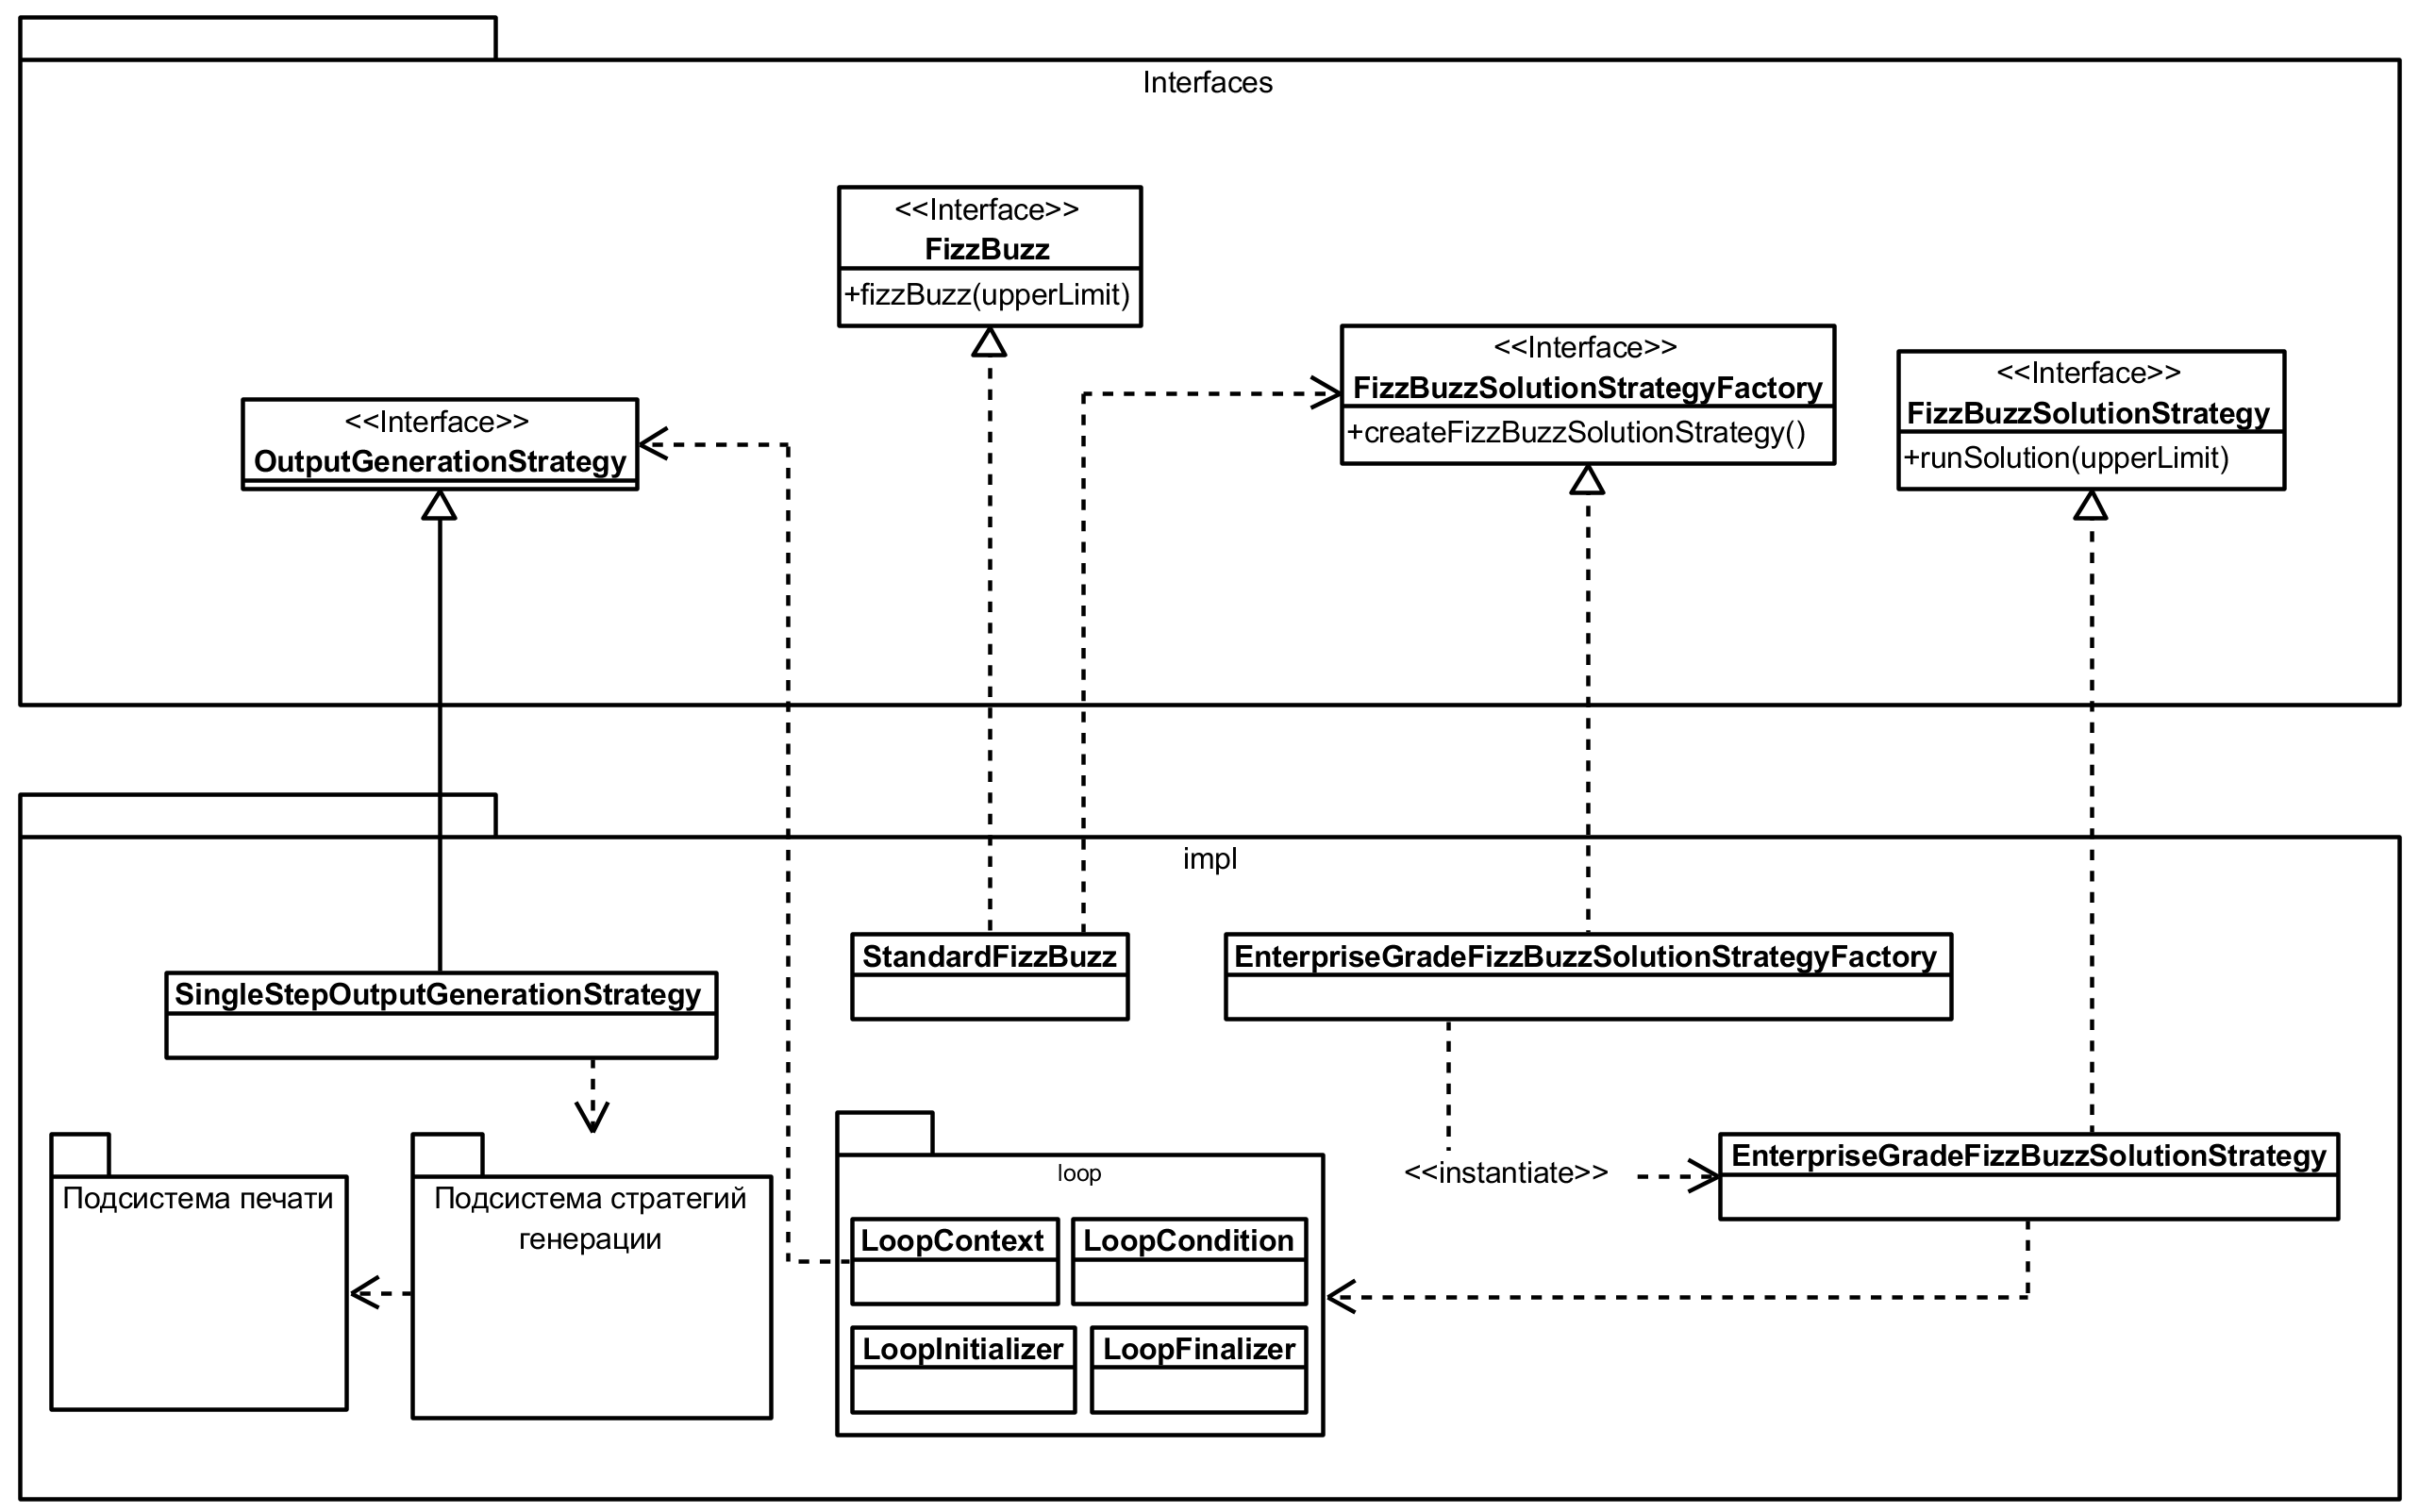
\includegraphics[width=\textwidth]{fizzBuzzArchitecture.png}
        \end{center}
    \end{frame}

    \begin{frame}
        \frametitle{Хорошие идеи}
        \begin{itemize}
            \item Separation of Concerns
            \item Dependency Inversion
            \item Dependency Injection
            \begin{itemize}
                \item Spring Framework
            \end{itemize}
            \item Паттерны ``Фабрика'', ``Стратегия'', ``Посетитель'', ``Адаптер'', что-то вроде паттернов ``Спецификация'' и ``Цепочка ответственности''
        \end{itemize}
    \end{frame}

    \begin{frame}
        \frametitle{Плохие идеи}
        \begin{itemize}
            \item Не выполняется принцип Keep It Simple Stupid
            \begin{itemize}
                \item Неправильно говорить ``строк кода написано'', правильно --- ``строк кода израсходовано''
            \end{itemize}
            \item ``Синтаксическое'' разделение на пакеты, а не ``семантическое''
            \begin{itemize}
                \item Отсутствие модульности, антипаттерн ``Big Ball of Mud''
            \end{itemize}
            \item Хардкод основных параметров вычисления
            \item Нет юнит-тестов, только интеграционные; нет логирования
            \item 1662 строки кода, очень мало комментариев (несмотря на принятый пуллреквест ``Serious Documentation'')
            \begin{itemize}
                \item Отсутствие архитектурного описания
            \end{itemize}
        \end{itemize}
    \end{frame}

    \section{Bash}

    \begin{frame}
        \frametitle{Bash\footnote{\tiny{По \url{http://aosabook.org}}}}
        \begin{itemize}
            \item Примерно 70К строк кода
            \item Исходный автор --- Brian Fox, maintainer --- Chet Ramey
            \item Первый релиз --- 1989
            \item Написан на C
            \item Архитектурное описание --- глава в \textit{The Architecture of Open Source Applications}, написанная Chet Ramey
        \end{itemize}
    \end{frame}

    \begin{frame}
        \frametitle{Архитектура Bash}
        \begin{center}
            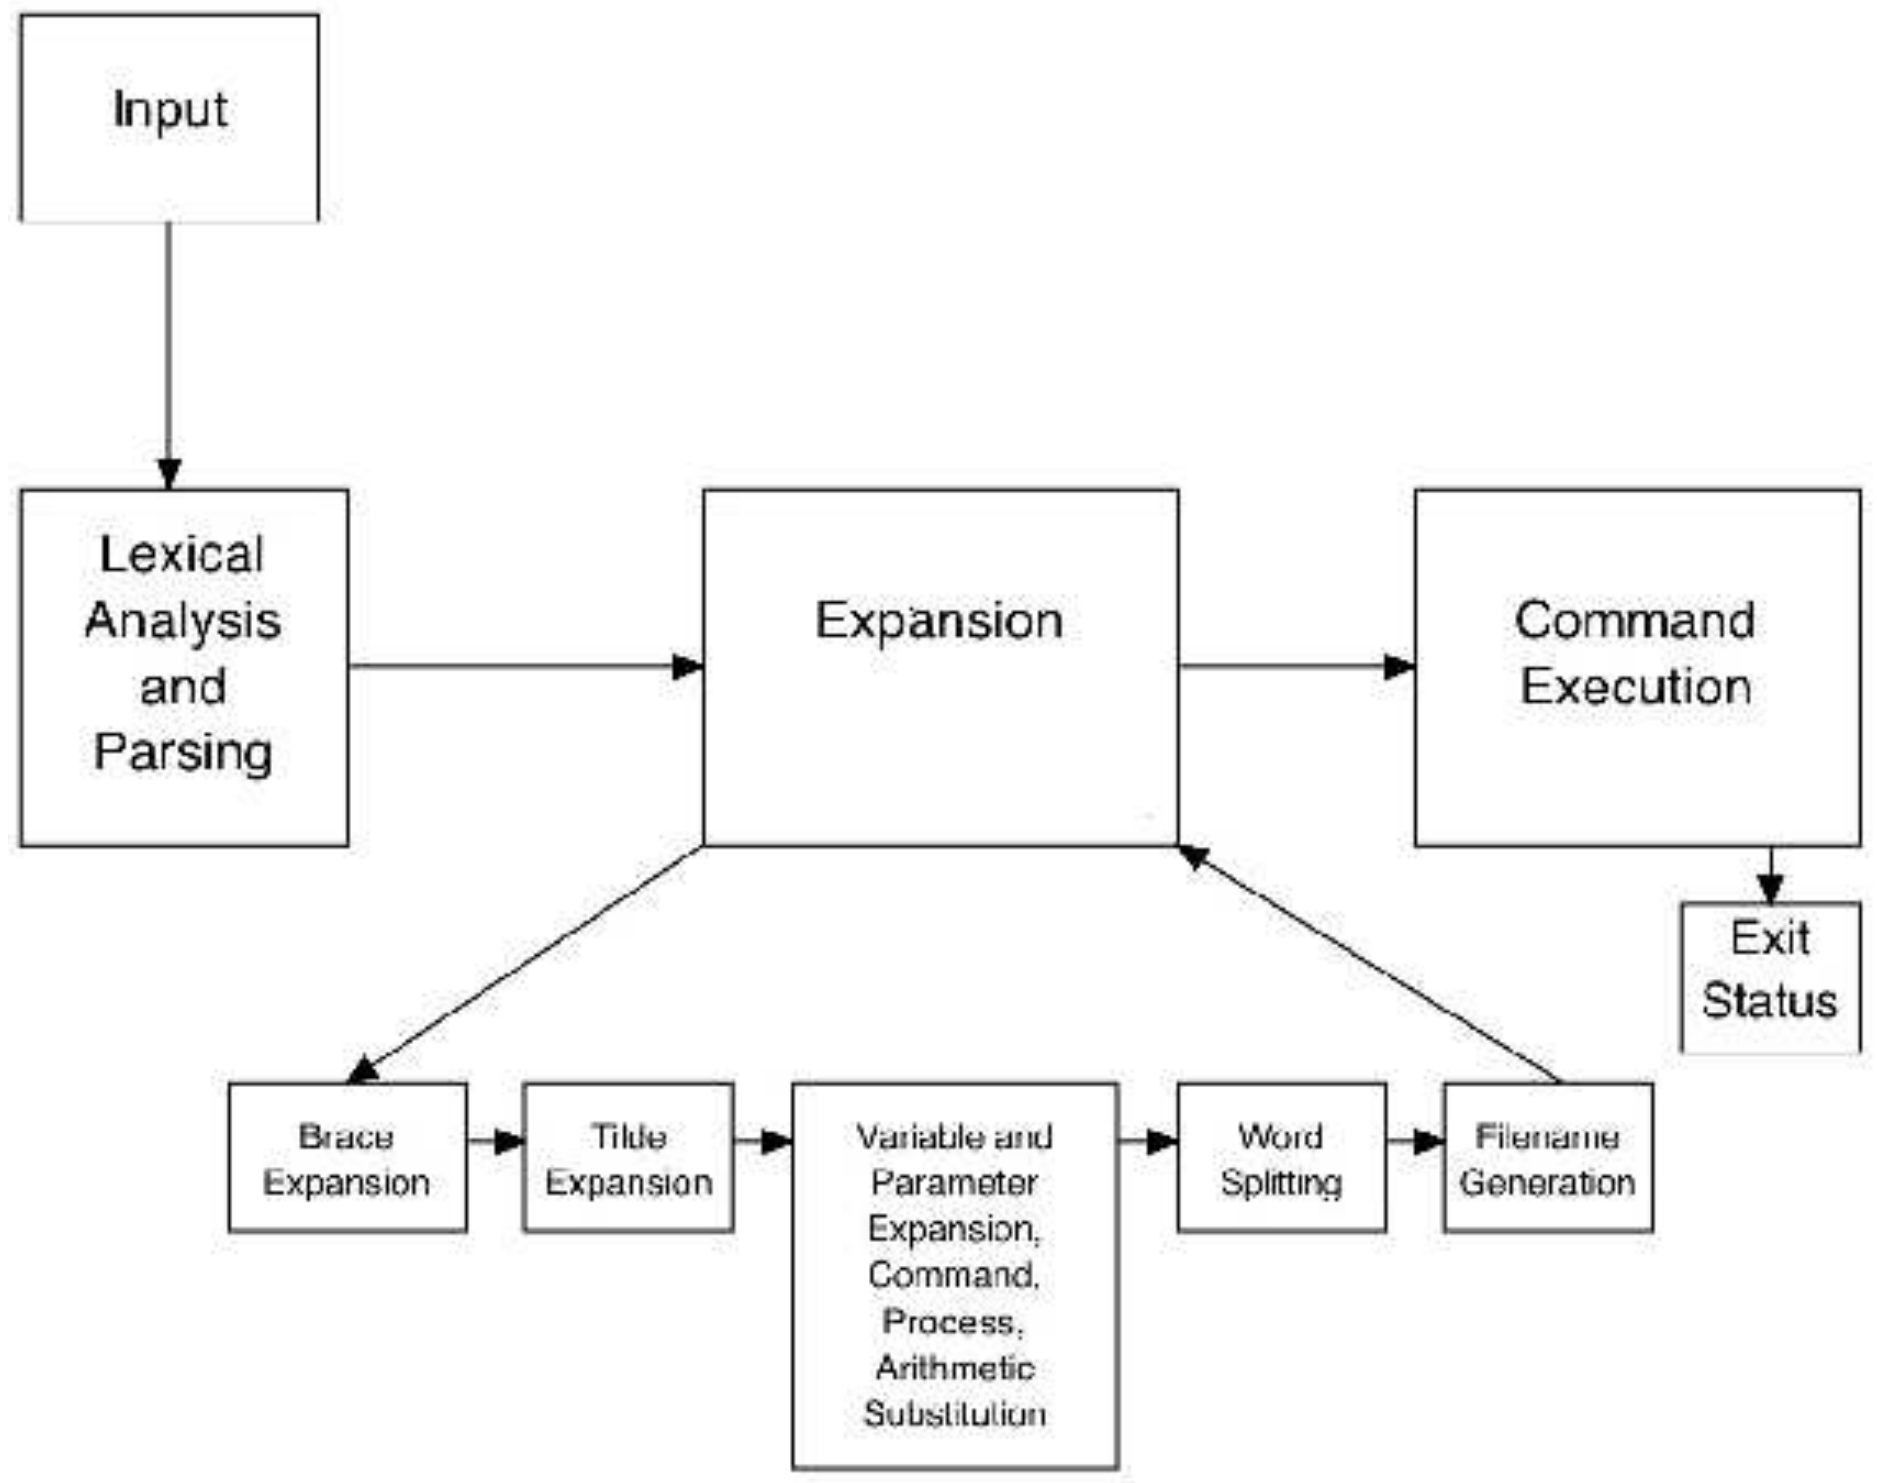
\includegraphics[width=0.7\textwidth]{bashArchitecture.png}
        \end{center}
    \end{frame}

    \begin{frame}[fragile]
        \frametitle{Основные структуры данных}
        \begin{minted}{c}
typedef struct word_desc {
    char *word; /* Zero terminated string. */
    int flags; /* Flags associated with this word. */
} WORD_DESC;
        \end{minted}

        \vspace{3mm}

        \begin{minted}{c}
typedef struct word_list {
    struct word_list *next;
    WORD_DESC *word;
} WORD_LIST;
        \end{minted}
    \end{frame}

    \begin{frame}
        \frametitle{Ввод с консоли}
        \begin{itemize}
            \item Библиотека Readline
            \begin{itemize}
                \item независимая библиотека, но пишется в основном для Bash
            \end{itemize}
            \item Цикл read/dispatch/execute/redisplay
            \item Dispatch table (или Keymap)
            \item Буфер редактирования, хитрый механизм расчёта действий для отображения
            \item Хранит все данные как 8-битные символы, но знает про Unicode
        \end{itemize}
    \end{frame}

    \begin{frame}[fragile]
        \frametitle{Синтаксический разбор}
        \begin{itemize}
            \item Зависимый от контекста лексический анализ
                \begin{minted}{sh}
for for in for; do for=for; done; echo $for
                \end{minted}
            \item Использует lex + bison
            \item Подстановка alias-ов выполняется лексером
            \item Сохранение и восстановление состояния парсера
        \end{itemize}
    \end{frame}

    \begin{frame}[fragile]
        \frametitle{Подстановки}
        \begin{minted}{sh}
${parameter:-word}
        \end{minted}

раскрывается в \textit{parameter}, если он установлен, и в \textit{word}, если нет

        \begin{minted}{sh}
pre{one,two,three}post
        \end{minted}

раскрывается в 

        \begin{minted}{sh}
preonepost pretwopost prethreepost
        \end{minted}

        Ещё бывает подстановка тильды и арифметическая подстановка, сопоставление шаблона
    \end{frame}

    \begin{frame}[fragile]
        \frametitle{Исполнение команд}
        \begin{itemize}
            \item Встроенные и внешние команды, обрабатываются единообразно
            \item Перенаправление ввода-вывода, отмена перенаправления
            \item Принимают набор слов
            \begin{itemize}
                \item Иногда обрабатывают по-особому, например, присваивание в \textit{export}
            \end{itemize}
            \item Присваивание --- тоже команда, но особая
            \item Перед запуском внешней команды --- поиск в PATH, кеширование результатов
            \item Job control, foreground и background
        \end{itemize}
    \end{frame}

    \begin{frame}[fragile]
        \frametitle{Lessons Learned}
        \begin{itemize}
            \item Комментарии к коммитам со ссылками на багрепорты с шагами воспроизведения
            \item Хороший набор тестов, в Bash их тысячи
            \item Стандарты, как внешние на функциональность шелла, так и на код
            \item Пользовательская документация
            \item Переиспользование
        \end{itemize}
    \end{frame}

    \section{Bash, на самом деле}

    \begin{frame}
        \frametitle{Архитектура Bash, на самом деле}
        \begin{itemize}
            \item J. Garcia et al., \textit{Obtaining Ground-Truth Software Architectures}
            \item 1 аспирант, 80 часов работы
            \item Верификация от Chet Ramey
            \item 70К строк кода, 200 файлов, 25 компонент
            \begin{itemize}
                \item 16 --- ядро, 9 --- утилиты
            \end{itemize}
            \item Структура папок почти не соответствует выделенным компонентам
        \end{itemize}
    \end{frame}

    \begin{frame}
        \frametitle{Архитектура Bash, на самом деле}
        \begin{center}
            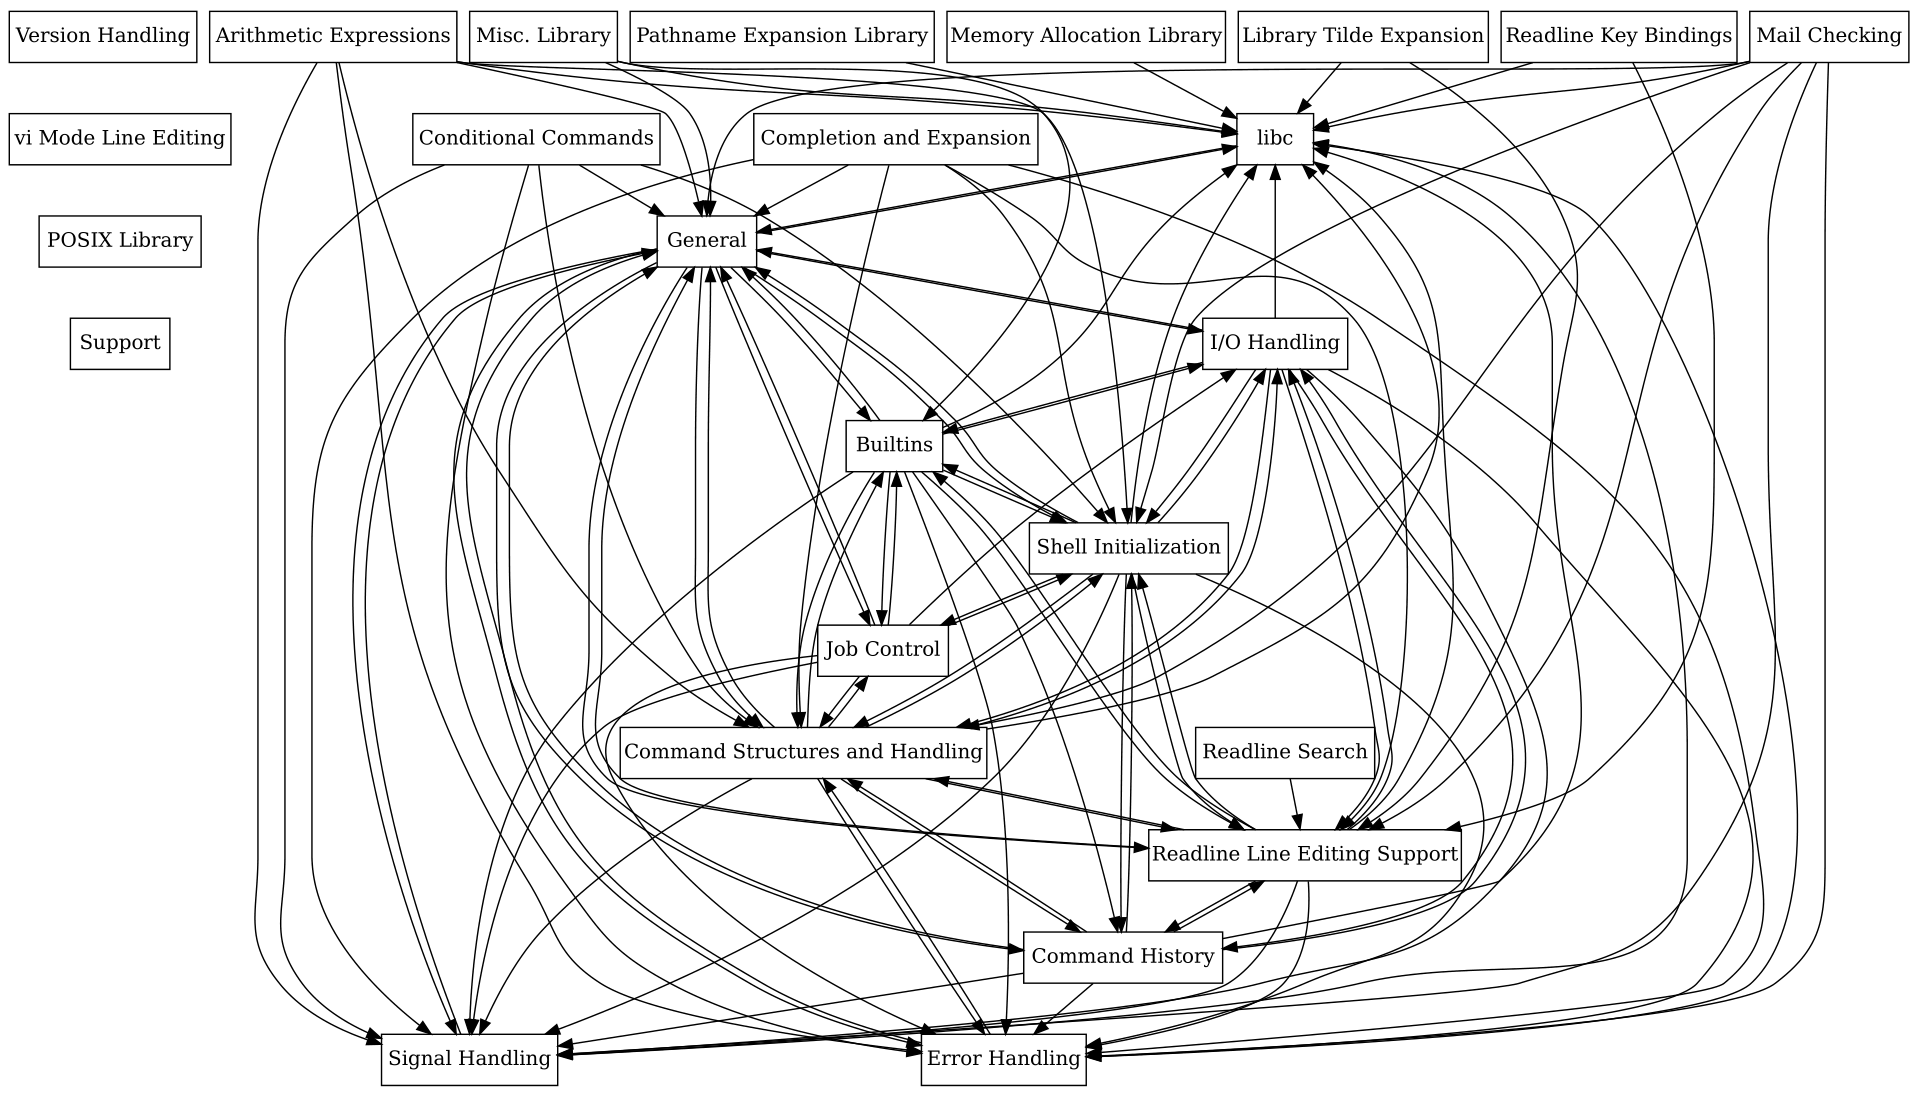
\includegraphics[width=\textwidth]{bashRealArchitecture.png}
        \end{center}
    \end{frame}

    \begin{frame}
        \frametitle{Результаты анализа кода}
        \begin{center}
            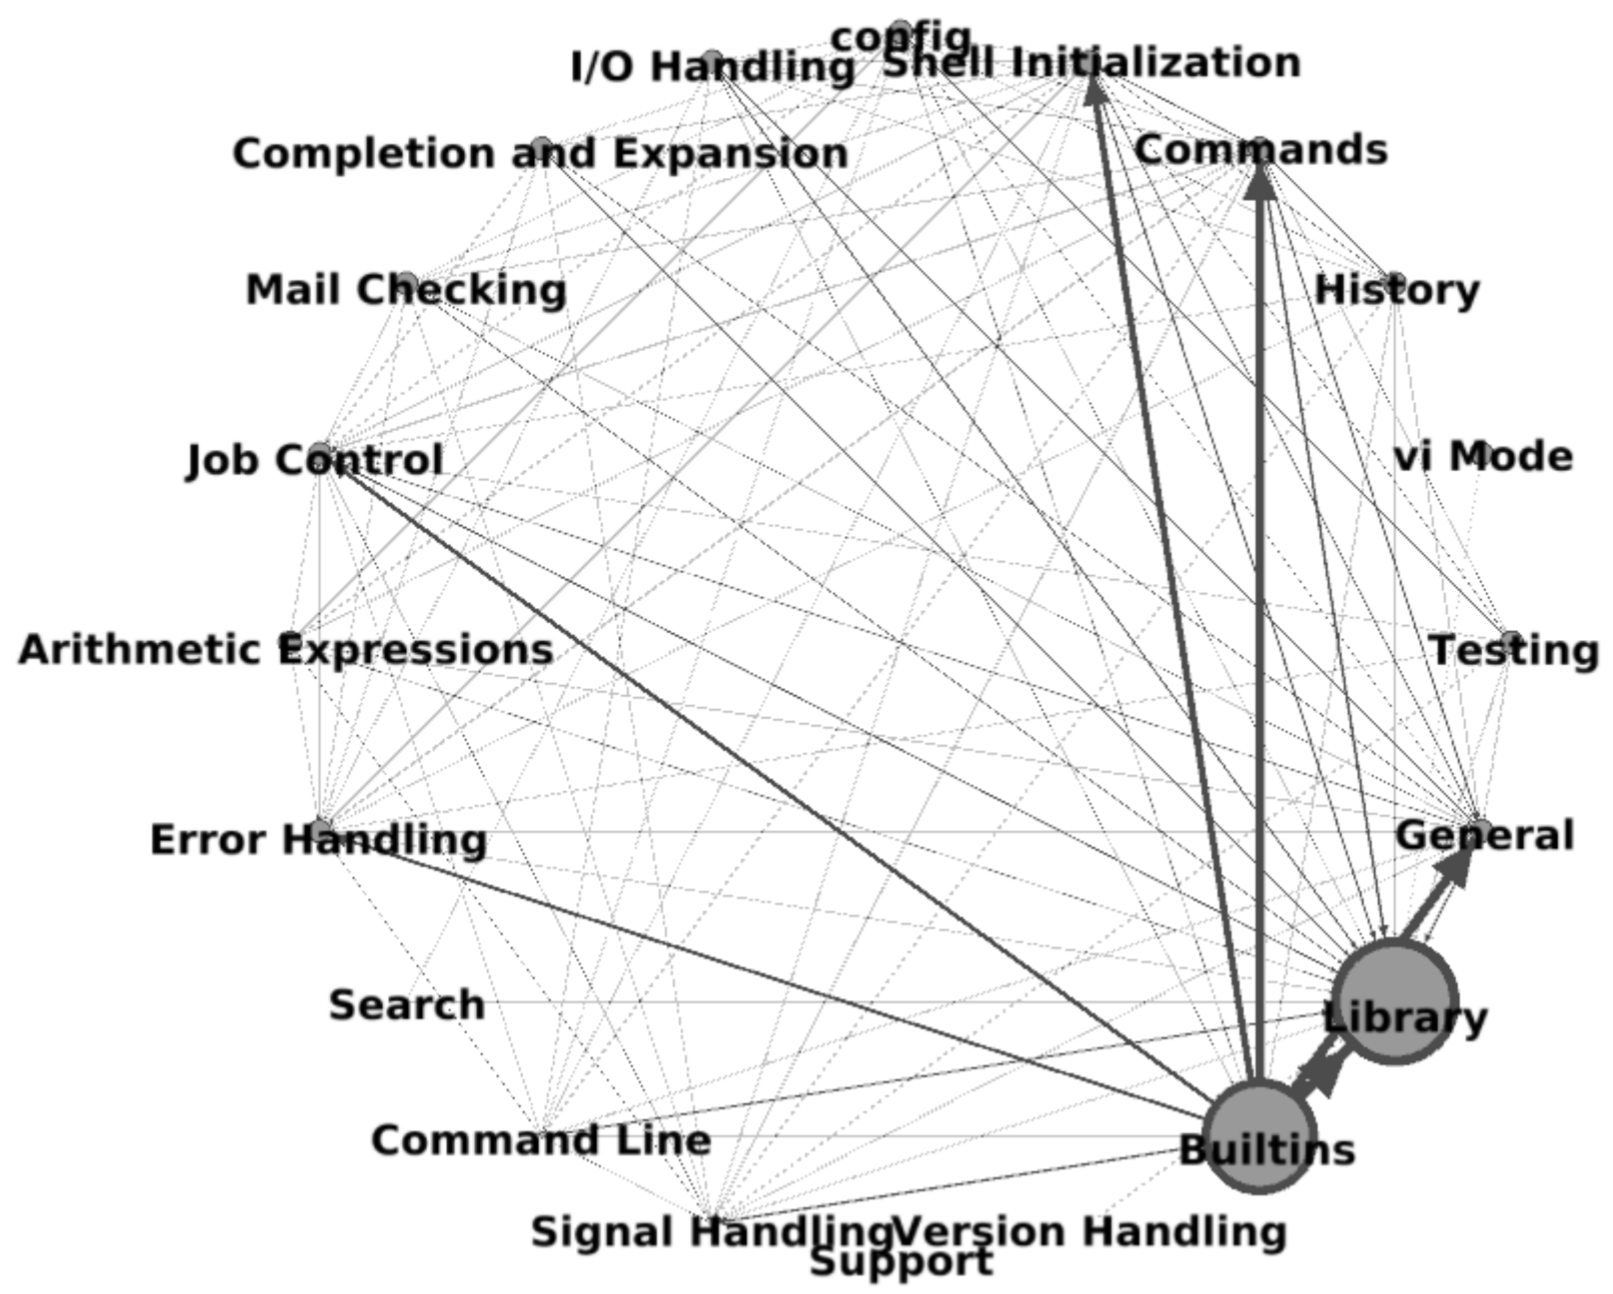
\includegraphics[width=0.7\textwidth]{bashAutomaticRecoveryArchitecture.png}
        \end{center}
    \end{frame}

    \begin{frame}
        \frametitle{Сравним с исходной}
        \begin{center}
            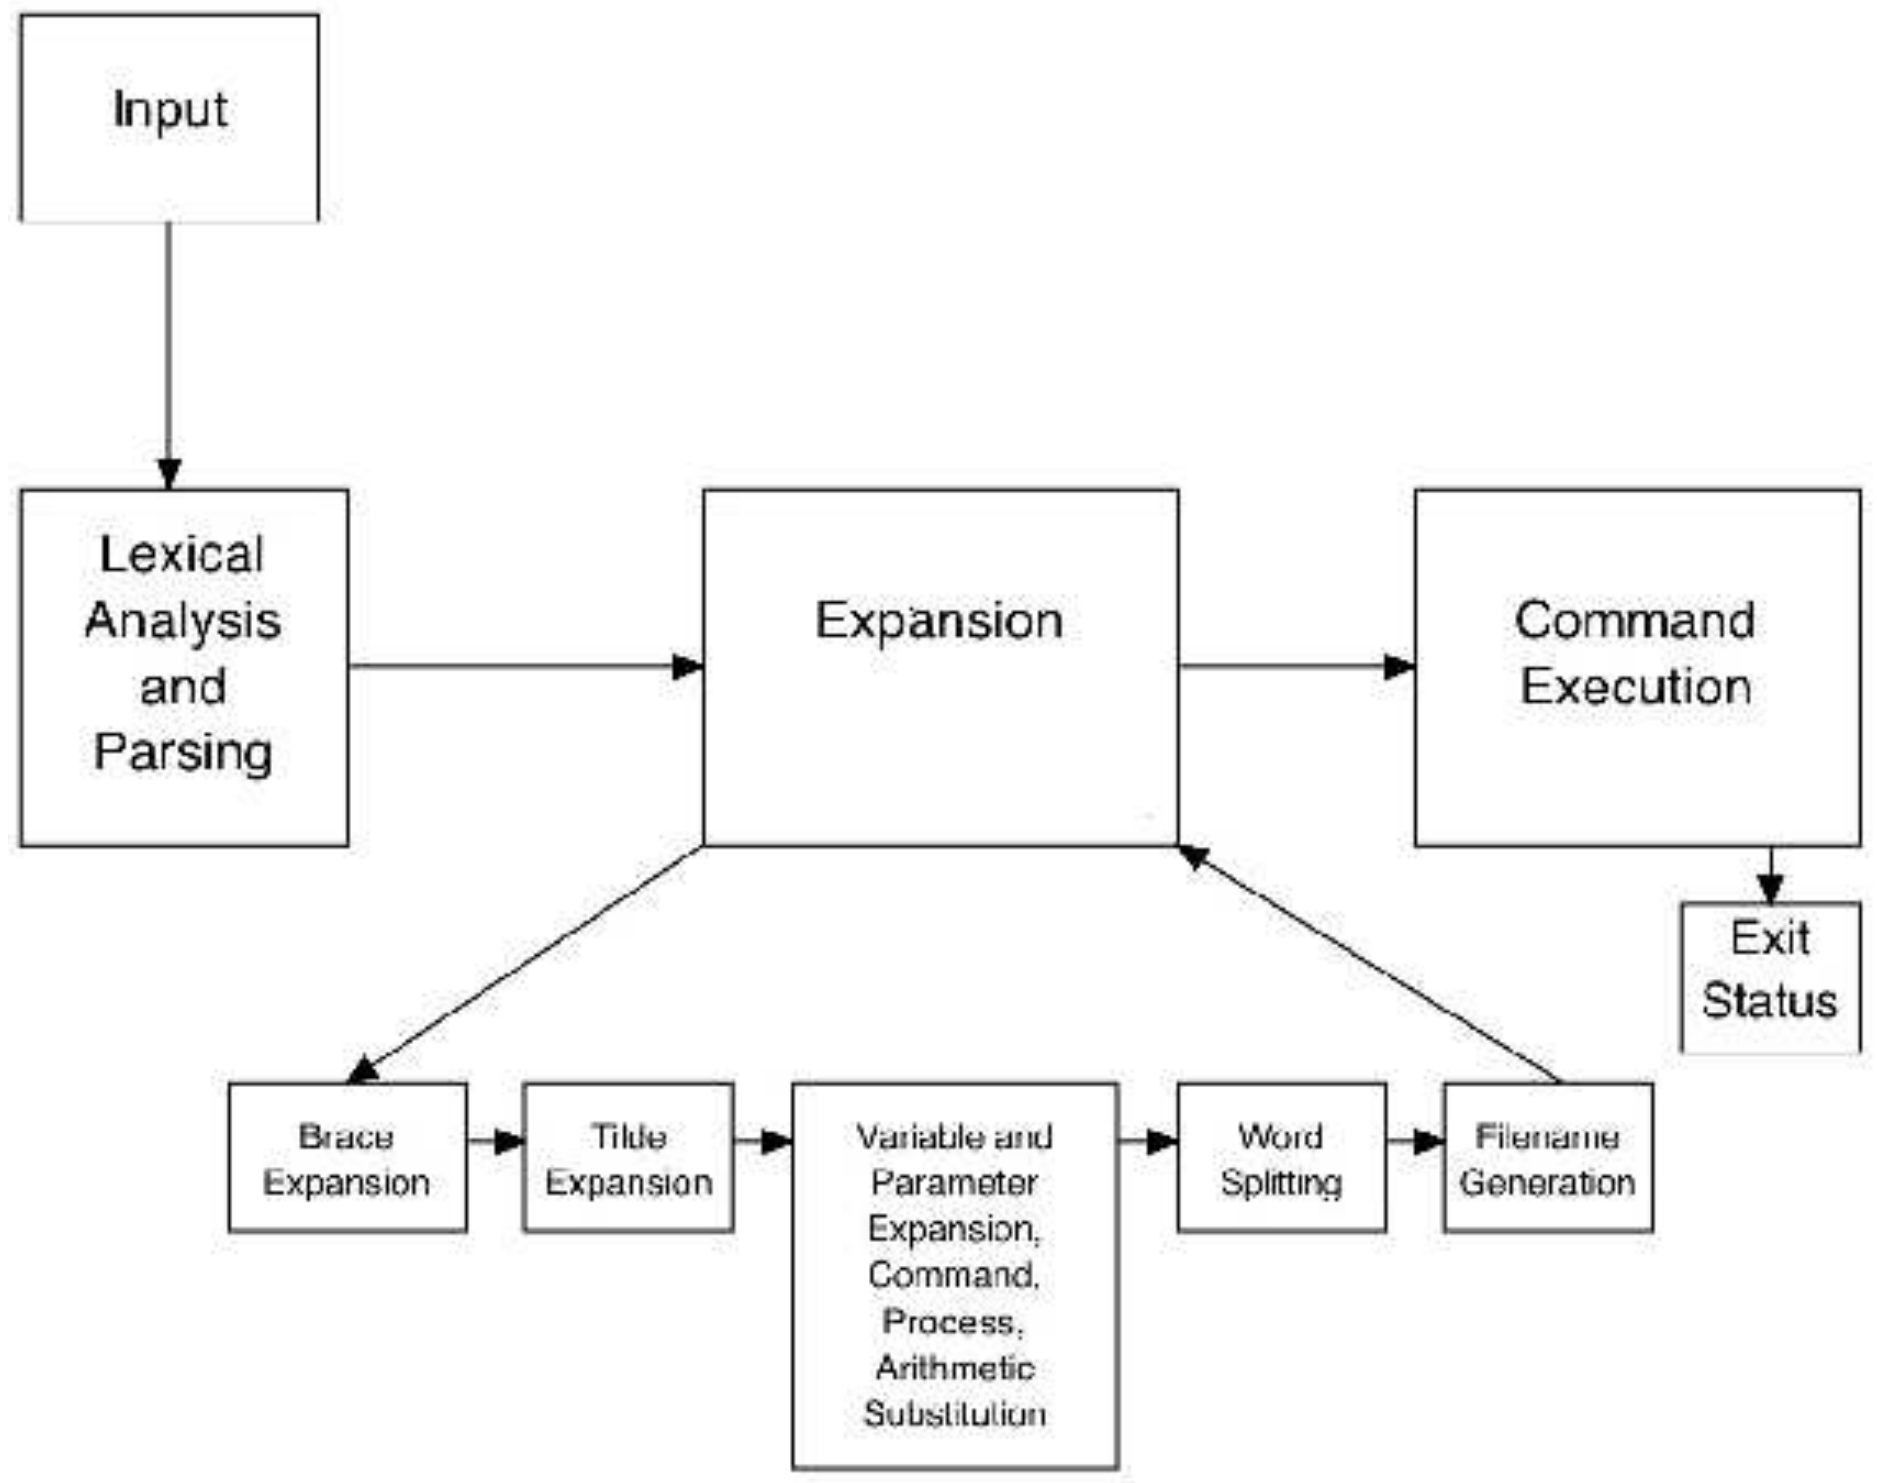
\includegraphics[width=0.7\textwidth]{bashArchitecture.png}
        \end{center}
    \end{frame}

    \begin{frame}
        \frametitle{Job Control}
        \begin{center}
            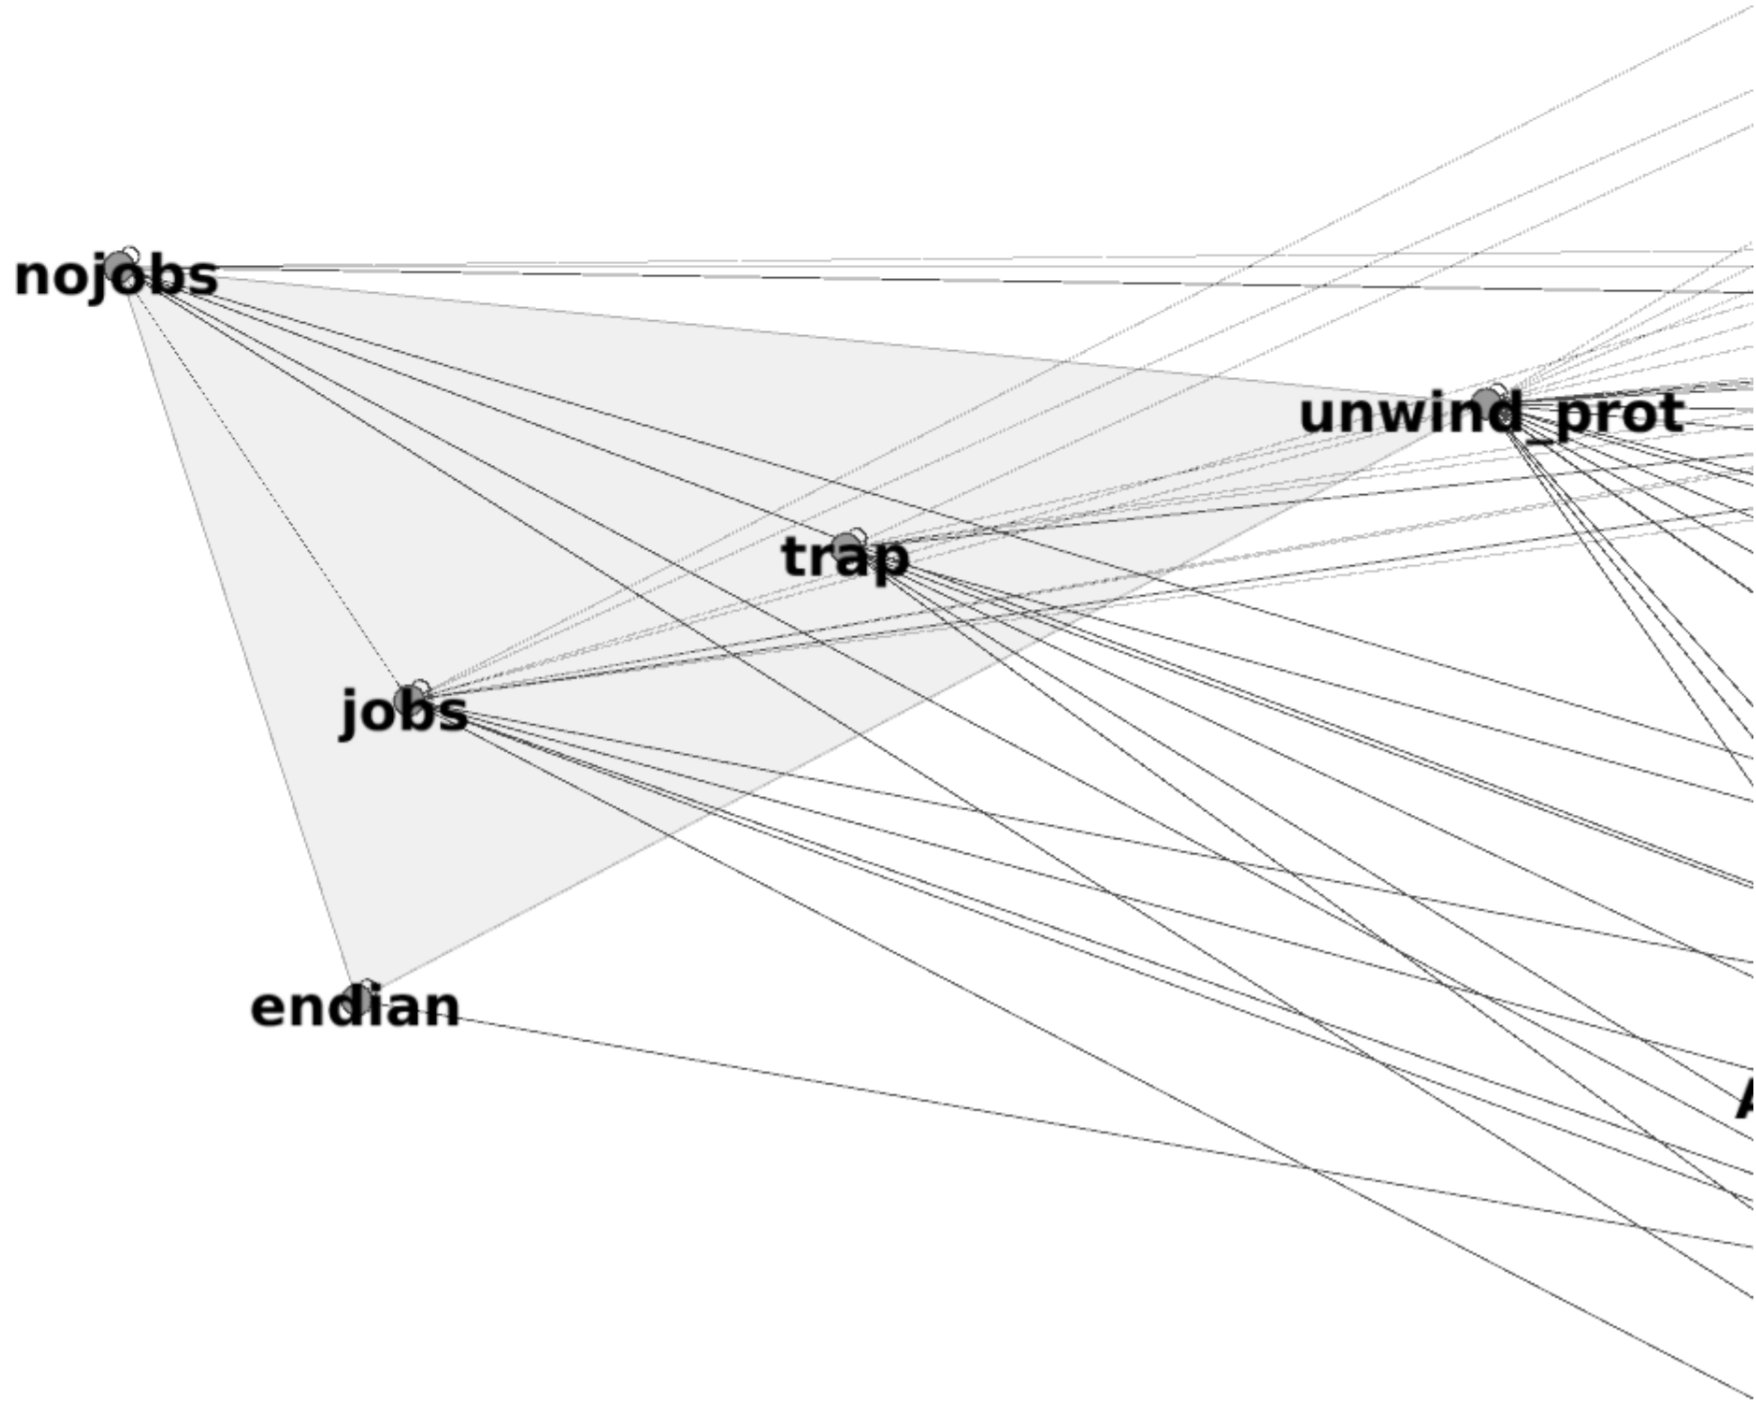
\includegraphics[width=0.7\textwidth]{bashJobControl.png}
        \end{center}
    \end{frame}

    \begin{frame}
        \frametitle{Commands}
        \begin{center}
            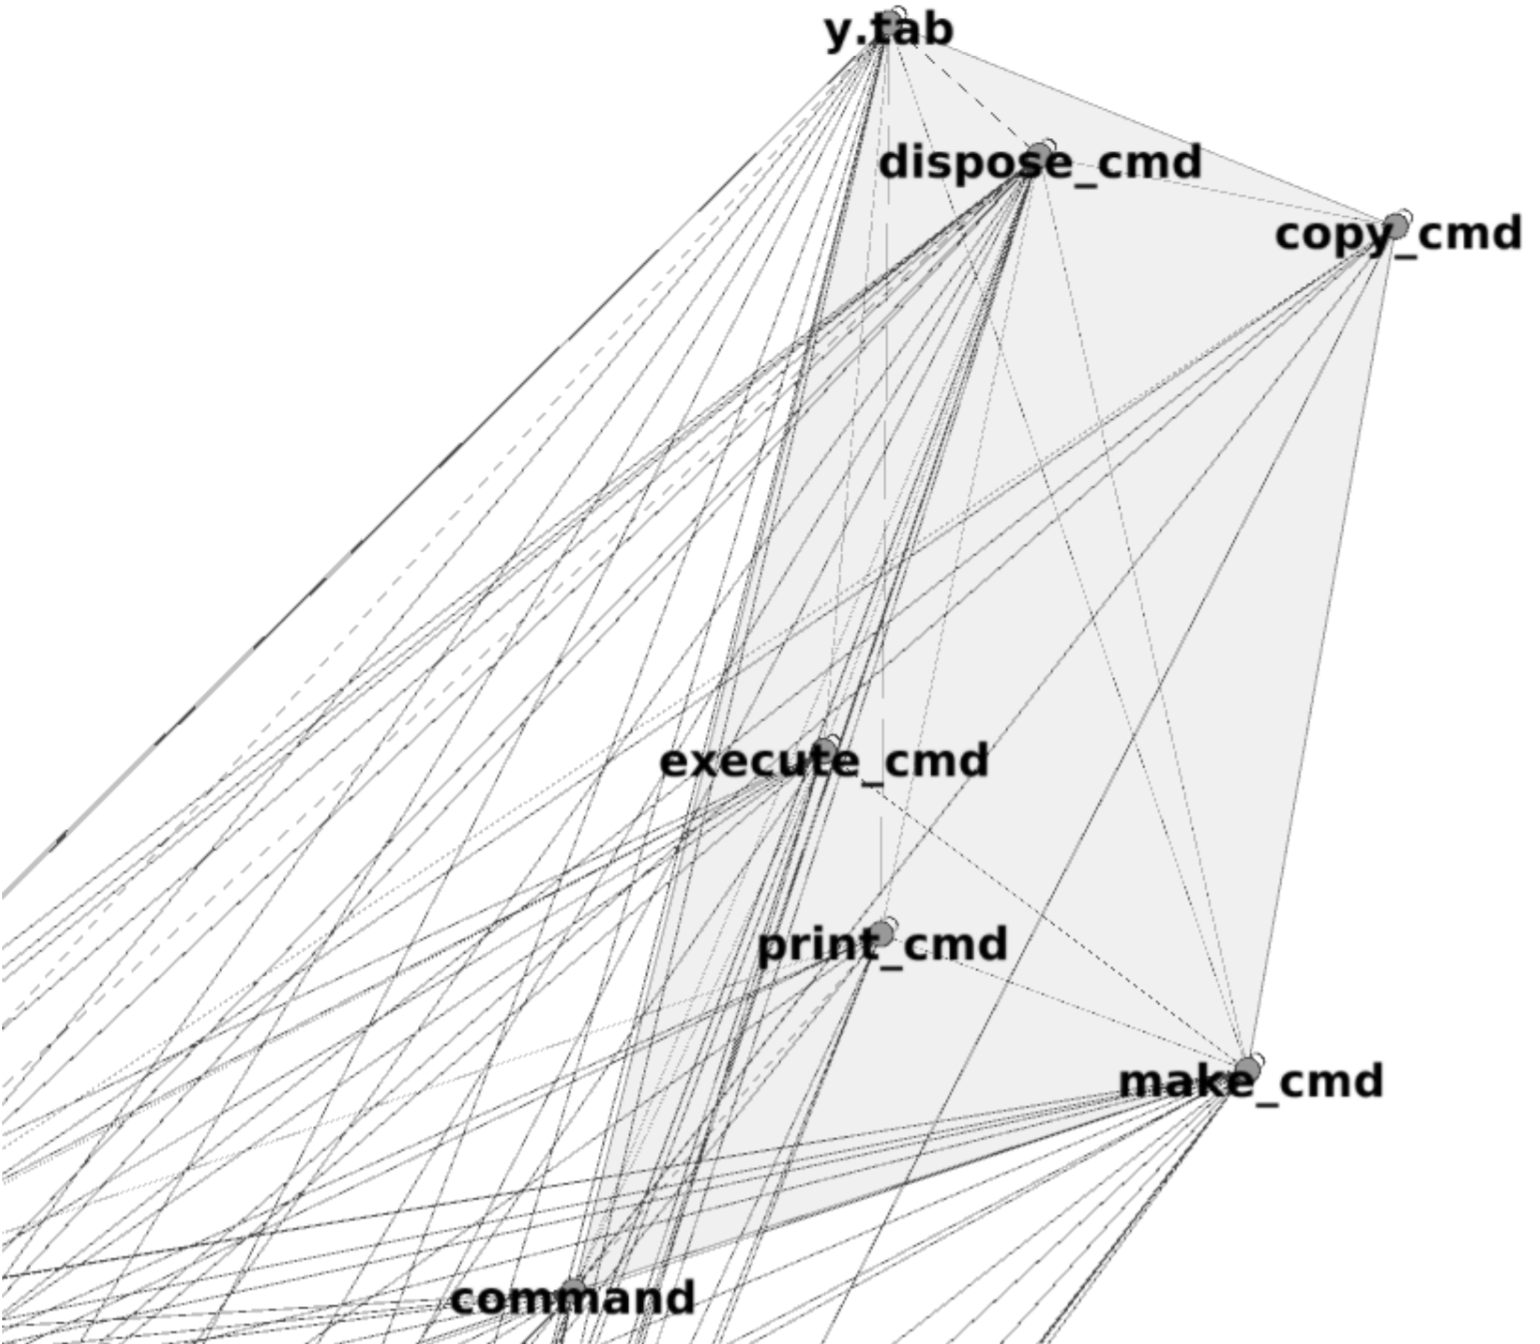
\includegraphics[width=0.7\textwidth]{bashCommands.png}
        \end{center}
    \end{frame}

    \section{Wesnoth}

    \begin{frame}
        \frametitle{Battle for Wesnoth\footnote{\tiny{По \url{http://aosabook.org}}}}
        \begin{columns}
            \begin{column}{0.4\textwidth}
                \begin{itemize}
                    \item Пошаговая стратегия
                    \item Порядка 200000 строк кода на C++
                    \item 4 миллиона скачиваний
                    \item 9/10 на Steam
                    \item 2003 год
                \end{itemize}
            \end{column}
            \begin{column}{0.6\textwidth}
                \includegraphics[width=\textwidth]{wesnoth.png}
                \attribution{https://www.wesnoth.org/}
            \end{column}
        \end{columns}
    \end{frame}

    \begin{frame}
        \frametitle{Architectural Drivers}
        \begin{itemize}
            \item Доступность для новых разработчиков и авторов контента
            \item В ущерб технической красоте
            \item Не nice to have, а условие выживания проекта в контексте широкого open-source сообщества из людей без каких-либо обязательств и разного технического уровня
        \end{itemize}
    \end{frame}

    \begin{frame}
        \frametitle{Высокоуровневая архитектура}
        \begin{columns}
            \begin{column}{0.6\textwidth}
                \begin{itemize}
                    \item Wesnoth Markup Language (WML)
                    \item Минимизация зависимостей от сторонних библиотек
                    \begin{itemize}
                        \item SDL (Simple Directmedia Layer) для видео и ввода/вывода
                        \begin{itemize}
                            \item Простота использования и кроссплатформенность
                        \end{itemize}
                        \item Boost, Pango, zlib, Python, Lua, GNU gettext
                    \end{itemize}
                \end{itemize}
            \end{column}
            \begin{column}{0.4\textwidth}
                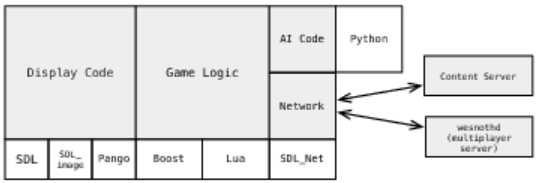
\includegraphics[width=\textwidth]{wesnothArchitecture.png}
            \end{column}
        \end{columns}
    \end{frame}

    \begin{frame}
        \frametitle{Основные компоненты}
        \begin{itemize}
            \item Парсер и препроцессор WML
            \item Базовый ввод-вывод --- видео, звук, сеть
            \item GUI --- виджеты
            \item Display module --- игровая доска, юниты, анимация и т.д.
            \item ИИ
            \item Поиск пути (плюс утилиты для работы с гексагональной доской)
            \item Генератор карт
            \item Специализированные модули
            \begin{itemize}
                \item Титульный экран
                \item Storyline module --- для проигрывания катсцен
                \item Лобби --- для мультиплеера
                \item ``Play game'' module --- управление основным игровым процессом
            \end{itemize}
            \item Отдельно --- wesnothd и content server
        \end{itemize}
    \end{frame}

    \begin{frame}[fragile]
        \frametitle{Wesnoth Markup Language}
        \begin{minted}{text}
[unit_type]
    id=Elvish Fighter
    name= _ "Elvish Fighter"
    image="units/elves-wood/fighter.png"
    hitpoints=33
    advances_to=Elvish Captain,Elvish Hero
    {LESS_NIMBLE_ELF}
    [attack]
        name=sword
        icon=attacks/sword-elven.png
        range=melee
        damage=5
    [/attack]
[/unit_type]
        \end{minted}
    \end{frame}

    \begin{frame}[fragile]
        \frametitle{Макросы}
        \begin{minted}{c++}
#define GOLD EASY_AMOUNT NORMAL_AMOUNT HARD_AMOUNT
  #ifdef EASY
    gold={EASY_AMOUNT}
  #endif
  #ifdef NORMAL
    gold={NORMAL_AMOUNT}
  #endif
  #ifdef HARD
    gold={HARD_AMOUNT}
  #endif
#enddef
...
{GOLD 50 100 200}
        \end{minted}
    \end{frame}

    \begin{frame}
        \frametitle{Модель данных}
        \begin{itemize}
            \item Всё сливается в один гигантский WML-документ
            \item Перезагружается при смене опций
            \item Всякие хаки на уровне препроцессора, чтобы не грузить вообще всё
            \item Классы unit и unit\_type (архитектурный стиль Knowledge Layer)
            \item Фиксированный набор поддерживаемых движком атрибутов, задаваемых для каждого типа через WML
            \begin{itemize}
                \item Нельзя описывать произвольное поведение через WML, хотели сохранить декларативность
            \end{itemize}
            \item Класс attack\_type
            \item Трейты, инвентарь
        \end{itemize}
    \end{frame}

    \begin{frame}
        \frametitle{Мультиплеер}
        \begin{itemize}
            \item Начальное состояние и команды
            \item Сервер просто пересылает команды между клиентами
            \begin{itemize}
                \item TCP/IP
            \end{itemize}
            \item Replay
            \item Никакой защиты от читов
            \item Версии клиентов
        \end{itemize}
    \end{frame}

    \begin{frame}
        \frametitle{Lessons Learned}
        \begin{itemize}
            \item 250 тысяч строк на WML
            \item Сотни созданных пользователями кампаний
            \item 74 тысячи коммитов, 196 контрибуторов
            \item Сами разработчики смеются над WML
            \item В целом задача обеспечить доступность для модификации очень сложна
        \end{itemize}
    \end{frame}

\end{document}
